\chapter{Conversor de base} \label{ch:basecvt}

\section{Objectius}

Volem fer un programa que permeti convertir nombres enters entre dues bases abitràries (fins a 36)
triades per l'usuari.
Per tant primer haurem de desenvolupar les rutines d'introducció de nombres i dissenyar com serà
la introducció de nombres en bases superiors a la decimal, ja que el teclat de la placa només té
digits, quatre lletres i dos símbols.

\section{Desenvolupament}

\subsection{Preliminars}

Abans de començar, implementarem una funció \fname{atoi} a \filename{util.c}
que fa el contrari a \fname{itoa}, és a dir, donat una cadena de caràcters
retorna el nombre al que correspon. La funció s'implementa així:

\begin{minted}{c}
int32_t atoi(const char *str, int32_t radix) {
    int k = 0, sign = 1;
    if (*str == '-' || *str == '+') {
        sign = (*str == '-') ? -1 : +1;
        str++;
    }
    for (; *str != '\0'; str++) {
        k *= radix;
        if (*str >= '0' && *str <= '9')
            k += *str - '0';
        else if (*str >= 'A' && *str <= 'Z')
            k += *str - 'A' + 10;
        else if (*str >= 'a' && *str <= 'z')
            k += *str - 'a' + 10;
    }
    return k * sign;
}
\end{minted}
\vskip -1em

Com que es tracta d'un programa complex i de més d'una rutina,
generarem dos fitxers \filename{baseconvert.c} i \filename{baseconvert.h}
on inserirem tot el codi.

\subsection{Disseny}

\paragraph{Introducció de nombres} El primer que hem de dissenyar és la introducció de nombres decimals enters.
L'usuari presionarà els digits que calgui, i podrà premer la tecla \texttt{*}
per esborrar l'últim caràcter o \texttt{\#} per entrar el nombre.

Com que no necessitem que puguin ser negatius, quan s'està introduint un nombre
només es reaccionarà quan es prenguin nous dígits, quan es premi \texttt{*}
i quan es premi \texttt{\#}.

Anem ara a la introducció de nombres en bases arbitràries. Quan la base és
decimal o més petita, podem simplement restringir els digits que calgui i tenir-ho
en compte al cridar \fname{atoi}. El problema és quan la base és major a 10.
En aquests casos es poden fer servir les lletres si la base és inferior a 14,
ja que les lletres es corresponen i la introducció segueix sent natural.

Ara bé, quan la base supera 14 no hi ha una forma natural, ni senzilla de
gestionar la introducció. Per permetre-ho igualment, si l'usuari vol, es
decideix el següent: la tecla \texttt{D} (la 'més alta') es podrà premer
varies vegades seguides per introduir lletres més altes. Per tant, si premem
\texttt{DD} tindrem una E, si premem \texttt{DDD} una F, i així mentre
la base escollida ho permeti. Quan es prem una tecla diferent a la \texttt{D}
s'enten que ja s'ha acabat d'introduir la lletra. Així doncs, \texttt{DADD2}
introduiria \texttt{DAE2}. Les tecles especials segueixen estant-hi; \texttt{*}
per esborrar l'últim caràcter o \texttt{\#} per entrar el nombre.

Ja tenim definida l'entrada de nombres. Ara definim com serà la interfície del
selector en general. Ho farem a partir d'una sessió d'exemple.

\paragraph{Introducció de les bases} En la primera fase, es pregunta a l'usuari per les dues bases entre les
que es vol convertir:

\begin{center}
  
\includegraphics[width=11em]{../\projectname/state-1} \\
  ( es prem \texttt{16} ) \\
  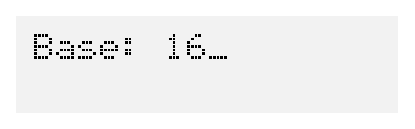
\includegraphics[width=11em]{../\projectname/state-2} \\
  ( es prem \texttt{\#} ) \\
  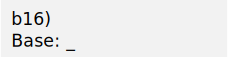
\includegraphics[width=11em]{../\projectname/state-3} \\
  ( es prem \texttt{2\#} ) \\
  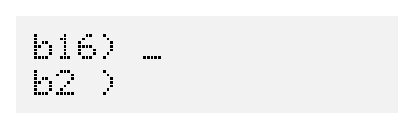
\includegraphics[width=11em]{../\projectname/state-4}
\end{center}

\paragraph{Conversió} Un cop ha introduit les dues, ens trobem en la segona fase on es poden introduir
nombres en la primera base i es mostra el resultat de la conversió cap a la segona base:

\begin{center}
  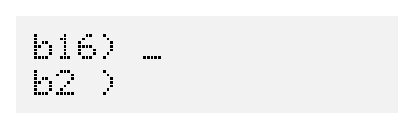
\includegraphics[width=11em]{../\projectname/state-4} \\
  ( es prem \texttt{1B} ) \\
  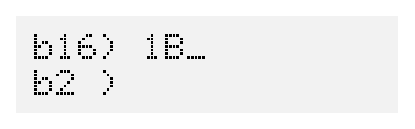
\includegraphics[width=11em]{../\projectname/state-5} \\
  ( es prem \texttt{\#} ) \\
  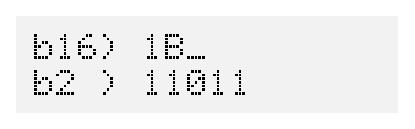
\includegraphics[width=11em]{../\projectname/state-6}
\end{center}

Podem editar el nombre i fer més conversions.

\paragraph{Canvi de selecció} També, si volem editar el nombre
\emph{en l'altre base}, podem girar l'encoder i llavors canviarem el cursor
d'edició a la línia de baix, on podem editar i llavors s'actualitza el nombre de dalt:

\begin{center}
  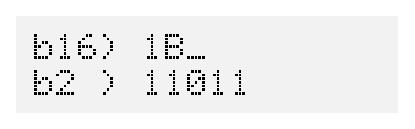
\includegraphics[width=11em]{../\projectname/state-6} \\
  ( $+$encoder ) \\
  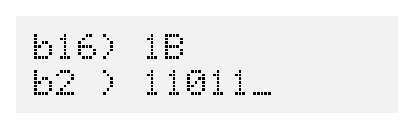
\includegraphics[width=11em]{../\projectname/state-7} \\
  ( es prem \texttt{*0} ) \\
  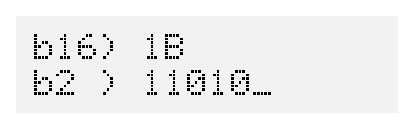
\includegraphics[width=11em]{../\projectname/state-8} \\
  ( es prem \texttt{\#} ) \\
  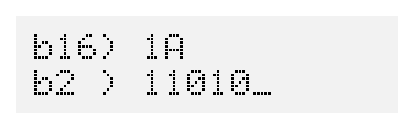
\includegraphics[width=11em]{../\projectname/state-9}
\end{center}

\paragraph{Canvi de base} Si esborrem tots els dígits prement \texttt{*} i llavors premem \texttt{\#},
podem canviar la base de la línia en la que ens trobem. Seguint amb la sessió d'exemple:

\begin{center}
  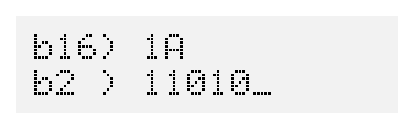
\includegraphics[width=11em]{../\projectname/state-9} \\
  ( es prem \texttt{*****} ) \\
  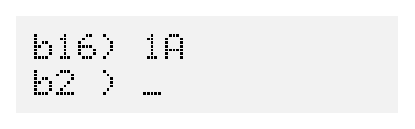
\includegraphics[width=11em]{../\projectname/state-10} \\
  ( es prem \texttt{\#} ) \\
  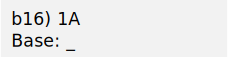
\includegraphics[width=11em]{../\projectname/state-11} \\
  ( es prem \texttt{10\#} ) \\
  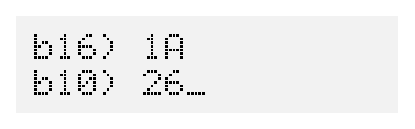
\includegraphics[width=11em]{../\projectname/state-12}
\end{center}

Com es pot veure, encara que canviem la base, la línia segueix mostrant el mateix nombre que abans (ara en la nova base).

% TODO: ellipsis


\subsection{Implementació}

En primer lloc implementarem les funcions per permetre a l'usuari
introduir text. Després aquest text el passarem a \fname{atoi} per
convertir-lo a nombre. La funció principal es defineix així:

\begin{minted}{c}
#define INPUT_CONTROLLER_MULTIPLE (1 << 9)

// Translation / validation function
// A function that, given a pressed key and the current string,
// returns a translated character or -1 if the pressed key
// isn't valid (inputs nothing), -2 if the string is complete,
// or -3 if delete last character (backspace).
// If a valid character is returned with INPUT_CONTROLLER_MULTIPLE bit set,
// the key is considered incompletely entered.
typedef int32_t (*InputController)(char *string, int32_t len, int32_t key, int32_t var, void *arg);

// Prompt the user for a string
//    string: variable to store input string in
//    len: initial length of string (i.e. how many characters are already input)
//    controller: key to character translation / validation function
//    col, row: column and row where the first character of the string is input
// Returns new string length
// - When calling this function, any already-input characters should be already
//   visible on the screen and any free area should be cleared
// - When this function has returned, the cursor is disabled again but the
//   LCD stays positioned at the end of the string. WAIT TILL KEY IS RELEASED!
// - Before return, a NUL terminator is added at the end of the string (not
//   included in returned length), but make sure the translator never returns 0.
//   Thus make sure string has space for maxLength + 1 characters.
// - Function can break if encoder changes, managed through encoderBreak:
//   pointer is set to true if we broke from encoder, not changed otherwise,
//   pass NULL to ignore encoder
int32_t enterString(char *string, int32_t len, int32_t maxLength,
        InputController controller, void* arg,
        int32_t col, int32_t row, int32_t *encoderBreak);
\end{minted}
\vskip -1em

Per ser genèrics i permetre fer servir la funció per a altres usos, es veu com la funció
delega part de la lògica de validació en un «controller» que li passem nosaltres. Aquest
controller és una funció que \fname{enterString} cridarà cada cop que es premi una tecla.
El controller decideix si la tecla és vàlida, i si ho és retorna el caràcter que li correspon.
El controller també pot retornar valors especials per indicar que la tecla te l'acció de
rectificar o d'acabar la introducció.

Aquesta és la implementació de \fname{enterString}:

\begin{minted}{c}
int32_t enterString(char *string, int32_t len, int32_t maxLength, InputController controller, void* arg, int32_t col, int32_t row, int32_t *encoderBreak) {
    // Enable cursor
    LCD_GotoXY(col + len, row);
    LCD_Config(TRUE, TRUE, FALSE);

    // Input loop
    int32_t incomplete_key, incomplete = 0;
    int32_t lastEncoder = encoderCount;
    while (1) {
        // Delay (to prevent chattering) and wait for key released
        DELAY_US(2000);
        while (readKeyboard() != KEY_NOT_FOUND);
        DELAY_US(2000);

        // Read key (TODO: timeout for incomplete key)
        int32_t key;
        do {
            key = readKeyboard();
            if (encoderBreak && (lastEncoder != encoderCount)) {
                *encoderBreak = 1;
                break;
            }
        } while (key == KEY_NOT_FOUND);

        // Before reacting, finish incomplete key if any
        if (incomplete > 0 && key != incomplete_key) {
            LCD_Config(TRUE, TRUE, FALSE);
            LCD_SendChar(string[len]);
            len++;
            incomplete = 0;
        }

        if (encoderBreak && *encoderBreak) break;

        // React to key
        int32_t ch = controller(string, len, key, incomplete, arg);
        if (ch == -2) {
            // Before returning, finish incomplete key if any
            if (incomplete > 0 && key != incomplete_key) {
                LCD_Config(TRUE, TRUE, FALSE);
                LCD_SendChar(string[len]);
                len++;
                incomplete = 0;
            }
            break;
        } else if (ch == -3) {
            // Before deleting, finish incomplete key if any
            if (incomplete > 0 && key != incomplete_key) {
                LCD_Config(TRUE, TRUE, FALSE);
                LCD_SendChar(string[len]);
                len++;
                incomplete = 0;
            }
            if (len > 0) {
                len--;
                LCD_GotoXY(col + len, row);
                LCD_SendChar(' ');
                LCD_GotoXY(col + len, row);
            }
        } else if (ch > 0) {
            if (len < maxLength) {
                // Write char to string
                string[len] = ch;
                LCD_SendChar(ch & 0xFF);
                len++;
                // Start (or continue) incomplete char
                if ((ch & INPUT_CONTROLLER_MULTIPLE) != 0) {
                    len--;
                    LCD_GotoXY(col + len, row);
                    LCD_Config(TRUE, FALSE, TRUE);
                    incomplete_key = key;
                    incomplete++;
                } else if (incomplete > 0) {
                    // Finish incomplete char
                    LCD_Config(TRUE, TRUE, FALSE);
                    LCD_SendChar(string[len]);
                    len++;
                    incomplete = 0;
                }
            }
        }
    }

    // Disable cursor and blink
    LCD_Config(TRUE, FALSE, FALSE);

    // Terminate string and return length
    string[len] = '\0';
    return len;
}
\end{minted}
\vskip -1em

De totes formes, s'ha implementat un controller que obeeix el funcionament que hem dit abans,
respecte a les lletres i les tecles especials. S'ha definit aixi:

\begin{minted}{c}
// Implementation of a controller allowing user to enter digits
// of a given radix (base). arg must point to an int32_t specifying
// the input radix between 2 and 36. To enter characters above D, user
// presses D repeatedly.
int32_t numberInputController(char *string, int32_t len, int32_t key, int32_t var, void *arg);
\end{minted}
\vskip -1em

S'ha implementat així:

\begin{minted}{c}
int32_t numberInputController(char *string, int32_t len, int32_t key, int32_t var, void *arg) {
    int32_t radix = *((int32_t*)arg);
    char ch = KEY_CHARS[key];

    // Handle first the case of D (incomplete) when radix > 14
    if (ch == 'D' && radix > 14) {
        // Return wraparound D-E-F-etc. depending on radix
        ch += var % (radix - 13);
        return INPUT_CONTROLLER_MULTIPLE | ch;
    }

    // Handle regular number / letter presses
    if (ch >= '0' && ch <= '9' && (ch - '0') < radix) return ch;
    if (ch >= 'A' && ch <= 'D' && (ch - 'A' + 0xA) < radix) return ch;

    // Other key presses
    if (ch == '*') return -3;
    if (ch == '#') return -2;
    return -1;
}
\end{minted}
\vskip -1em

Finalment, una funció \emph{helper} que crida a la primera i la combina amb \fname{atoi}
per retornar el nombre introduit ja parsejat:

\begin{minted}{c}
static inline int32_t enterNumber(char *string, int32_t *len, int32_t maxLength, int32_t radix, int32_t col, int32_t row, int32_t *encoderBreak) {
    *len = enterString(string, *len, maxLength, numberInputController, &radix, col, row, encoderBreak);
    return (*len > 0) ? atoi(string, radix) : -1;
}
\end{minted}
\vskip -1em

% TODO: provide examples, split here into two sections

Ara que ja tenim la capa d'entrada, la resta del programa s'implementa així:

\begin{minted}{c}
/** PROGRAM **/

typedef struct {
    int32_t radix;
    int32_t maxLength;
    char line [LCD_COLUMNS+1];
    char string [32]; // at worst case has to fit 31 binary digits + NUL
    int32_t len;
    int32_t overflow;
} ConversionBucket;

static void setBucket(ConversionBucket *bucket, int32_t n);

static void initBucket(ConversionBucket *bucket, int32_t n, int32_t row) {
    int32_t col;

    // Clear row
    LCD_GotoXY(0, row);
    for (col = 0; col < LCD_COLUMNS; col++)
        LCD_SendChar(' ');

    // Input base
    LCD_GotoXY(0, row);
    LCD_SendString("Base:");

    char string [3];
    int32_t len = 0, radix = -1;
    while (!(radix >= 2 && radix <= 36))
        radix = enterNumber(string, &len, 2, 10, 6, row, NULL);

    // Calculate maximum length for source base input
    // length can not be longer than floor( 31 / log2(base) )
    uint32_t maxLength = 0, current = 1;
    while (TRUE) {
        uint32_t next = current * (uint32_t)radix;
        if (next / (uint32_t)radix != current || (current & BIT31)) break;
        current = next;
        maxLength++;
    }

    // Set bucket parameters
    bucket->radix = radix;
    bucket->maxLength = maxLength;

    // Render static line part
    col = 0;
    bucket->line[col++] = 'b';
    col += strlen(itoa(radix, &bucket->line[col], 10));
    while (col < 3)
        bucket->line[col++] = ' ';
    bucket->line[col++] = 2;
    while (col < LCD_COLUMNS)
        bucket->line[col++] = ' ';
    bucket->line[LCD_COLUMNS] = 0;

    // Set bucket number
    setBucket(bucket, n);
}

static void setBucket(ConversionBucket *bucket, int32_t n) {
    // If no number provided, empty string
    if (n == -1) {
        bucket->string[0] = 0;
        bucket->len = 0;
        bucket->overflow = 0;
        return;
    }

    // Convert n to string at our radix
    itoa(n, bucket->string, bucket->radix);
    bucket->len = strlen(bucket->string);
    bucket->overflow = 0;

    // If string too long, put ellipsis at the end
    if (bucket->len > (LCD_COLUMNS - 4)) {
        bucket->len = LCD_COLUMNS - 4 - 1;
        bucket->string[bucket->len] = 0;
        bucket->overflow = 1;
    }
}

static void renderBucket(ConversionBucket *bucket, int32_t row) {
    LCD_GotoXY(0, row);
    LCD_SendString(bucket->line);
    LCD_GotoXY(4, row);
    LCD_SendString(bucket->string);
    if (bucket->overflow) {
        LCD_GotoXY(LCD_COLUMNS-1, row);
        LCD_SendChar(3);
    }
}

static int32_t promptBucket(ConversionBucket *bucket, int32_t row, int32_t *encoderBreak) {
    return enterNumber(bucket->string, &bucket->len, bucket->maxLength, bucket->radix, 4, row, encoderBreak);
}

void baseConverter(void) {
    // Initialize LCD
    LCD_Config(TRUE, FALSE, FALSE);
    static const uint8_t separator [] = {
        0b00000000,
        0b00000100,
        0b00000110,
        0b00011111,
        0b00000110,
        0b00000100,
        0b00000000,
        0b00000000,
    };
    LCD_CustomChar(2, separator);
    static const uint8_t ellipsis [] = {
        0b00000000,
        0b00010000,
        0b00011100,
        0b00011111,
        0b00011100,
        0b00010000,
        0b00000000,
        0b00000000,
    };
    LCD_CustomChar(3, ellipsis);

    // Initialize (ask for base) on both buckets
    int32_t n = -1;
    static ConversionBucket buckets [2];
    initBucket(&buckets[0], n, 0);
    renderBucket(&buckets[0], 0);
    initBucket(&buckets[1], n, 1);
    renderBucket(&buckets[1], 1);

    // Repeatedly ask on one bucket, set value
    int32_t lastEncoder = encoderCount;
    int32_t sel = 0;
    while (1) {
        int32_t encoderBreak = 0;
        int32_t input = promptBucket(&buckets[sel], sel, &encoderBreak);
        if (encoderBreak) {
            int32_t encoderDiff = encoderCount - lastEncoder;
            lastEncoder += encoderDiff;
            sel += encoderDiff;
            if (sel < 0) sel = 0;
            if (sel > 1) sel = 1;
            continue;
        }
        if (input == -1) {
            initBucket(&buckets[sel], n, sel);
            renderBucket(&buckets[sel], sel);
        } else {
            n = input;
            int32_t i;
            for (i = 0; i < 2; i++) {
                setBucket(&buckets[i], n);
                renderBucket(&buckets[i], i);
            }
        }
    }
}
\end{minted}
\vskip -1em

La funció principal és \fname{baseConverter}. Com podem veure, el bucle principal
és super petit, la majoria del codi està en els altres mètodes. A més es defineix un
\emph{conversion bucket}, que representa una de les dues línies de conversió amb la
seva base i nombre actuals. Els mètodes actuen sempre sobre un \emph{conversion bucket}.

El codi es carrega a la placa i es comprova el correcte funcionament.
Treient de banda millores estètiques, s'ha respectat el disseny establert en el primer apartat. 

\section{Conclusió}

S'ha realitzat sense problemes, i tot i que crec que el resultat final no
és tan intuitiu com tenia en ment, estic satisfeta amb el resultat.

\section{Ajustaments posteriors}

Cap.
